\documentclass{beamer}
\usetheme{Hannover}
\usefonttheme{serif}
\usepackage{graphicx}
\usepackage{algpseudocode}
\usepackage{subfig}
\usepackage{mathrsfs}
\usepackage{xspace}
\newcommand{\A}{\texttt{A}}
\newcommand{\G}{\texttt{G}}
\newcommand{\U}{\texttt{U}}
\newcommand{\C}{\texttt{C}}
\newcommand{\klf}{\textsc{k-Local Folding}\xspace}
\newcommand{\rf}{\textsc{Nussinov}\xspace}
\newcommand{\s}{\vspace{1cm}}
\newcommand{\al}{\mathscr{A}}
\renewcommand{\qedsymbol}{$\blacktriangleleft$}

\title{\klf}
\subtitle{A Local Alignment Approach to RNA folding}
\author{Ben Chugg, Coulter Beeson, Kenny Drabble, Jeff Jeyachandren}
\institute{\textsc{The University of British Columbia}}
\date{April 6,2017}

\begin{document}
\begin{frame}
\titlepage
\end{frame}


\begin{frame}
\section*{Background}
\frametitle{RNA Folding}
RNA consists of the four base pairs Adenine (\A), Guanine (\G) , Cytosine (\C) and Uracil (\U). These base pairs of RNA pair in a complementary fashion: Adenine to Uracil ($\A-\U$) and Cytosine to Guanine ($\C-\G$). \\

Unlike DNA for which we are concerned with optimally aligning two strands, for RNA we are concerned with how the strand folds with itself. 

\begin{figure}
\centering
\includegraphics[scale=0.07]{images/hairpin_loop.png}
\vspace{-0.2cm}
\caption{Source: \url{http://rosalind.info/problems/pmch/}}
\end{figure}
\end{frame}

\begin{frame}
\frametitle{RNA Folding}
There are several frameworks with which we can model RNA folding. We will use the Energy Minimization Model. \s

In this model, matches are scored as $+1$ and non-matches as 0. This lends itself to a dynamic programming algorithm: Nussinov's algorithm which we will call \rf. 
\end{frame}

\begin{frame}
\frametitle{RNA Folding}
Let $r=r_1,\ldots,r_n$ be a strand of RNA, where $r_i\in\{\A,\C,\G,\U\}$ and let $S(i,j)$ denote the optimal score of folding the subsequence $s_i,s_{i+1}\ldots s_j\subset s$. Then, 
\[S(i,j)=\max\begin{cases}
S(i+1,j-1)+1,&\text{if }i,j\text{ base pair}\\
S(i+1,j),\\
S(i,j-1),\\
\displaystyle \max_{i<k<j}\{S(i,k)+S(k+1,j)\},&\text{bifurcation}.
\end{cases}\]

It's clear that the runtime is $O(n^3)$. 
\end{frame}


\begin{frame}
\section{Our Approach}
\frametitle{\klf}
\rf returns the mathematically optimal alignment under the energy minimization model. Therefore, any new approach cannot hope to beat the scores, but only improve the running time. \s

\textbf{Idea}: Subsequences of an RNA strand which are (near) palindromes of each other are likely to be a good match. Pair these regions and pass the leftover segments to \rf. 
\end{frame}

\begin{frame}
\frametitle{\klf}
\textbf{Formal Goal:} We propose a heuristic based approach to speed up Nussinov with a fast preprocessing step. \s

Formally, we define an algorithm \klf which takes as input an RNA strand $r$ and a parameter $k$, runs a local alignment algorithm on the strand to find $k$ high scoring --- and disjoint --- palindromic regions of $r$. It then passes the remaining unpaired regions to \rf to be folded as usual.
\end{frame}

\begin{frame}
\frametitle{\klf} 
\begin{algorithmic}[1]
\Procedure{k-Local Folding}{$r,k$}
\State Initialize stack $S\gets r$
\While{The number of local alignments found is $\leq k$ and $S$ not empty}
\State $s\gets \text{pop}(S)$
\State Let $\overline{s}$ be the reverse of $s$
\State Call Local Alignment on $s$ and $\overline{s}$.
\If{Local alignment found}
\State Remove the aligned regions from $s$
\State Push all unmatched regions of $s$ back onto stack
\EndIf 
\EndWhile
\State Call \rf on all unmatched regions of $r$. 
\EndProcedure
\end{algorithmic}
\end{frame}

\begin{frame}
\frametitle{\klf}
\begin{block}{example}
\begin{figure}
\centering
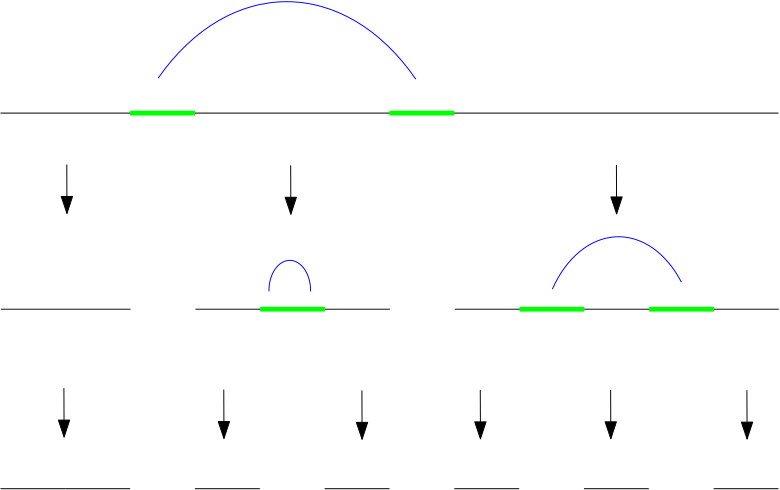
\includegraphics[scale=0.28]{images/k_local_sequence.png}
\caption{A strand of RNA undergoing multiple local alignments on successive subsequences. The unmatched regions at the bottom will be passed into \rf}. 
\end{figure}
\end{block}
\end{frame}

\begin{frame}
\subsection{Runtime Analysis}
\frametitle{\klf: Runtime Analysis}
Fix an RNA strand $r$ with length $n$. 
\begin{lemma}[1]
Let $\al$ be the set of local alignments found. Finding $k$ disjoint local alignments of $r$ takes time $O(n^2 k)$. 
\end{lemma}
\begin{lemma}[2]
\klf runs in time
\[O\left(\left(n-\sum_{A\in\al}\ell_A\right)^3+n^2k\right),\] where $\ell_A$ is the length of an alignment $A\in\al$. 
\end{lemma}
\end{frame}

\begin{frame}
\begin{proof}[Proof of Lemma 1]
We can view the progress of the algorithm as a ternary tree: amortized across each level we perform local alignment on a sequence of size $n-\sum_{A\in\al}\ell_A$. Local alignment takes time squared in the size of the input. Since the tree in the worst case has depth $k$, the result follows. 
\end{proof}
\begin{proof}[Proof of Lemma 2]
Running \rf takes cubic time in the size of the input. \klf first finds $k$ disjoint alignments, then runs \rf on the remaining unmatched regions, which have total length $n-\sum_{A\in\al}\ell_A$.   The result follows by applying lemma 1. 
\end{proof}
\end{frame}

\begin{frame}
\frametitle{How big is the tree?}
\begin{block}{remark}
It's a very unlikely case that the depth of the tree is $k$: it will more likely be $\log(k)$. Therefore, an average case analysis will yield that \klf runs in time 
\[O\left(\left(n-\sum_{A\in\al}\ell_A\right)^3+n^2\log (k)\right).\]
\end{block}
\end{frame}

\begin{frame}
\frametitle{$k$-Local Folding: Runtime Analysis}
We remark that since $\sum_{A\in\ell_A}\ell_A^3\in O(n^3)$, $O((n-\sum_{A\in\al}\ell_A)^3)=O(n^3)$ so there is no asymptotic difference between \klf and \rf.
However, our hypothesis was that there may a difference in the run times in practice.  

\begin{block}{example}
In the extreme case, suppose $r$ is a perfect palindrome. Then we do $O(n^2)$ work instead of $O(n^3)$, so we gain a factor of $n$. 
\end{block}
\end{frame}

\begin{frame}
\section{Results}
\subsection{Runtimes}
\frametitle{Results: Runtimes} 
Each trial was run with 20 random sequences, and the results were taken as the average of those trials. 
The following data is for 16S Ribosomal Subunit RNA. 
\begin{figure}
\centering
\subfloat[$k\in\{0,1,\ldots,10\}$]{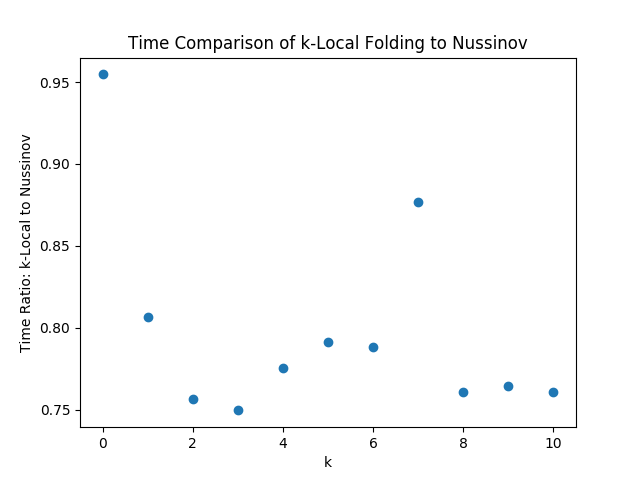
\includegraphics[scale=0.32]{../figures/TIME_k0-10_20seqs_rna.png}}
\subfloat[$k\in\{14,\ldots,20\}$]{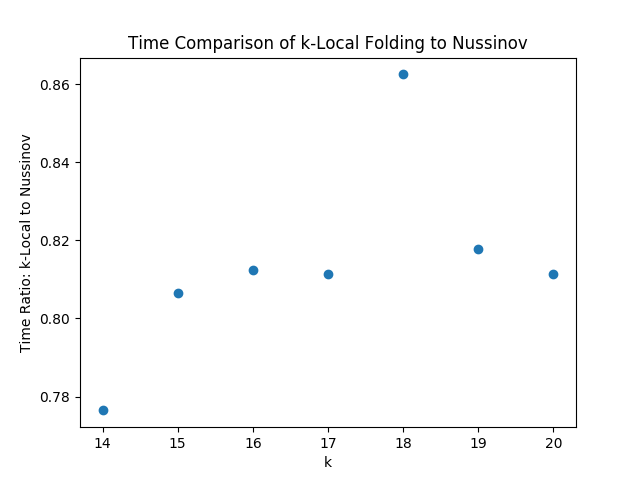
\includegraphics[scale=0.32]{../figures/TIME_k14-20_20seqs_rna.png}}
\end{figure}
\end{frame}

\begin{frame}
\frametitle{Results: Runtimes}
Ciliate Telomerase RNA data.
\begin{figure}
\subfloat[$k\in\{0,\ldots,10\}$]{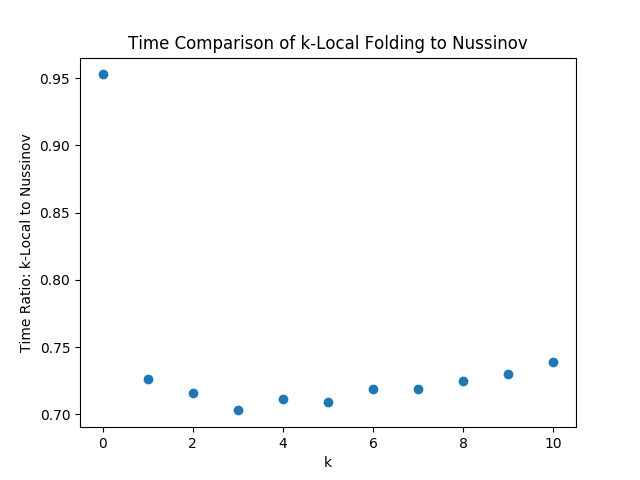
\includegraphics[scale=0.32]{../figures/TIME_k0-10_20seqs_ciliateRna.png}}
\subfloat[$k\in\{14,\ldots,20\}$]{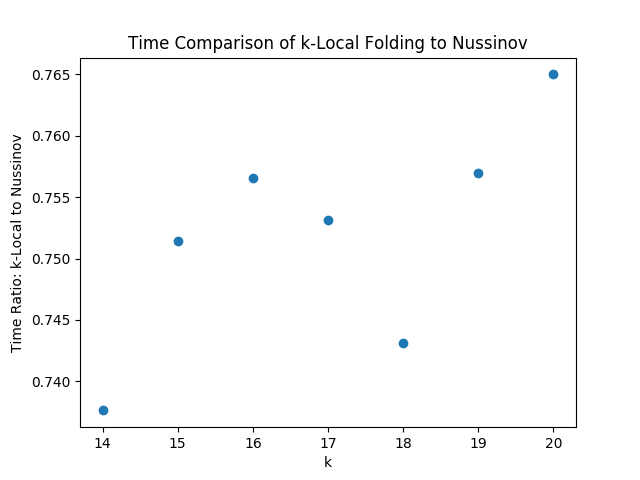
\includegraphics[scale=0.32]{../figures/TIME_k14-20_20seqs_ciliateRna.png}}
\end{figure}
\end{frame}


\begin{frame}
\subsection{Scores}
\frametitle{Results: Scores}
16s Ribosomal Subunit RNA
\begin{figure}
\centering
\subfloat[$k\in\{0,\ldots,10\}$]{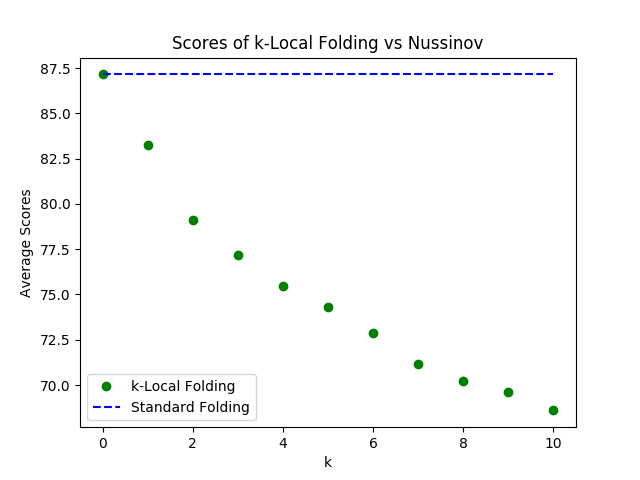
\includegraphics[scale=0.32]{../figures/SCORE_k0-10_20seqs_rna.png}}
\subfloat[$k\in\{14,\ldots,20\}$]{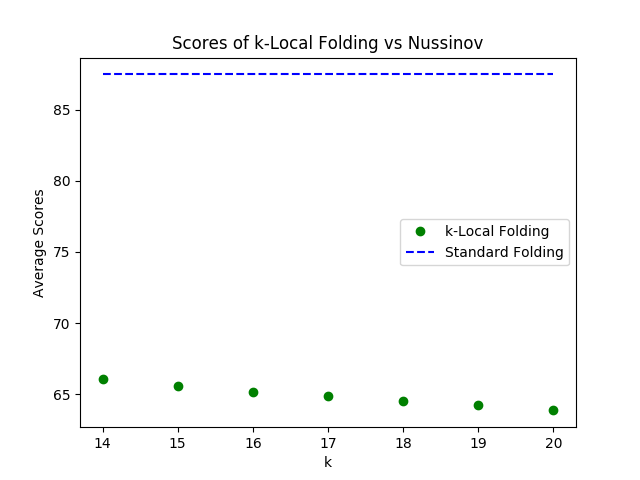
\includegraphics[scale=0.32]{../figures/SCORE_k14-20_20seqs_rna.png}}
\end{figure}
\end{frame}


\begin{frame}
\frametitle{Results: Runtimes}
Ciliate Telomerase RNA data.
\begin{figure}
\subfloat[$k\in\{0,\ldots,10\}$]{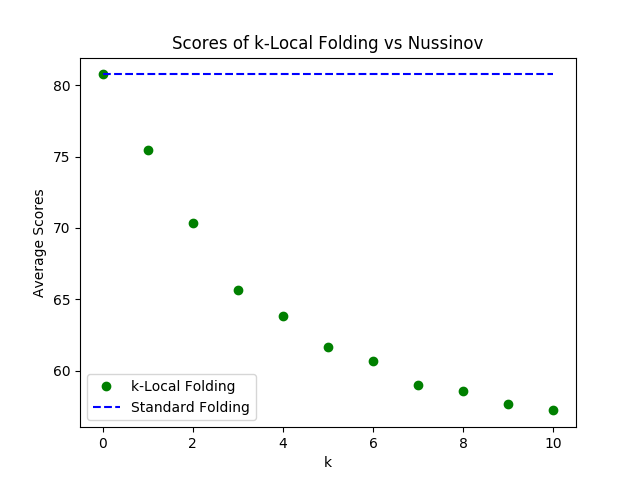
\includegraphics[scale=0.32]{../figures/SCORE_k0-10_20seqs_ciliateRna.png}}
\subfloat[$k\in\{14,\ldots,20\}$]{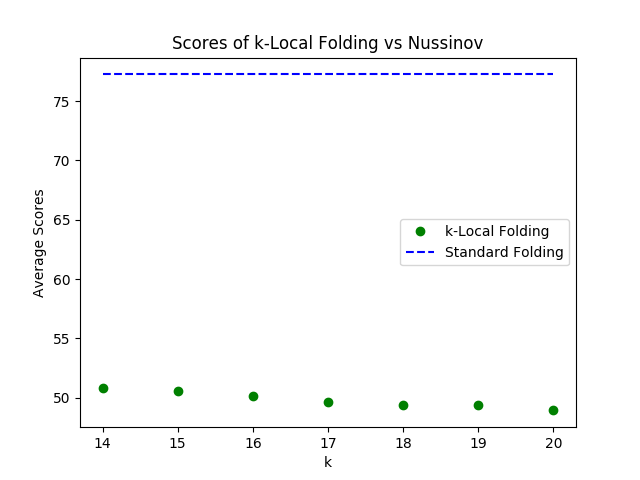
\includegraphics[scale=0.32]{../figures/SCORE_k14-20_20seqs_ciliateRna.png}}
\end{figure}
\end{frame}


\begin{frame}
\section{Conclusion}
\frametitle{Concluding Remarks}
\begin{enumerate}
\item Results look fairly invariant under different data. 
\item \klf may be best used as a preprocessing step for traditonal  RNA folding algorithms for regions which are likely hairpinned. 
\end{enumerate}
\end{frame}


\begin{frame}
\section{Extensions}
\frametitle{Extensions and Further Research}
\begin{enumerate}
\item Can we speed up \klf by being smarter with our data structures? Tempting to only do local alignment once ... 
\item Modify \klf to report possible pseudoknots 
\item Implement \klf to use the Four Russians speedup of \rf. 
\item  Probabilistic (Viterbi-like) Approach
\item Providing better bounds on the runtime based on the expected number of palindromic like regions found on an alignment. 
\end{enumerate}
\end{frame}

\begin{frame}
The code and slides can be found at \url{https://github.com/bchugg/bwt}. 
\end{frame}

\end{document}